

\section{Introduction}

Analyzing the performance of a complicated application is challenging, since an application frequently interacts with multiple components inside the system, such as different libraries, the operating system, or the underlying hardware. Any mismatch between any components therein may cause the application to suffer substantial performance losses.
%Whenever one component is not tapped with applications very well, then the performance of such applications can be greatly impacted. 

A memory allocator is a component that could significantly impact the performance of applications, due to multiple reasons. First, many applications perform extensive invocations of allocations and deallocations via the memory allocator. Since memory management is on the critical path, the allocator's memory management operations will greatly affect the application that is using this allocator.
Second, even if an allocator is efficient in its management operations, it could still cause significant slowdown if it is not application-friendly, such as when suffering from a serious false-sharing issue. Fig.~\ref{fig:motivation} shows such an example. TcMalloc is a well-known performant allocator that was designed by Google~\cite{tcmalloc}, however it is running $47\times$ slower than the default Linux allocator for \texttt{cache-thrash}, due to a false-sharing issue. 

%with a low cache utilization rate. In case of low cache utilization rate, there will be more program stalls in the execution caused by waiting for the data loading from the memory, comparing to the one with high cache utilization rate.  

%Performance of modern applications is often greatly impacted by memory accesses. when obtaining undesired performance, programmers mainly focus on optimizing the program code. Although memory allocators serve as the sole proxy for programs to request and return memory from the operating system, programmers lack even basic understandings of their behaviors, such as how well they perform themselves, how they interact with the OS, and whether their memory management policy fits the target program. 

In order to investigate the performance impact, we evaluated the following allocators, including two Linux allocators (glibc-2.28 and glibc-2.21), TcMalloc~\citep{tcmalloc}, \texttt{jemalloc}~\citep{jemalloc}, Hoard~\citep{Hoard}, DieHarder~\citep{DieHarder}, and OpenBSD's allocator~\citep{openbsd}, where the latter two are secure allocators. We ran the same set of applications from PARSEC~\citep{parsec}, Phoenix~\citep{phoenix}, and multiple synthetic applications from Hoard~\cite{Hoard}, and observed the dramatic performance difference among them. Fig.~\ref{fig:motivation} shows performance results of partial applications, where all data in the figure are normalized to the runtime of the Linux default allocator. We have the following observations: (1)~the performance difference with different allocators can be as large as $88\times$, indicating that sometimes spending additional effort toward optimizing the application code may have a smaller performance impact than simply switching to a better-suited allocator. (2~No allocator performs consistently the best across all tested applications, indicating the importance of confirming whether an allocator is suitable for a particular application. 

%\todo{Xin: Use the gprof{} and Coz to try on one application--dedup, check whether they could identify the issues inside or not. }


\begin{figure}[!ht]
\centering
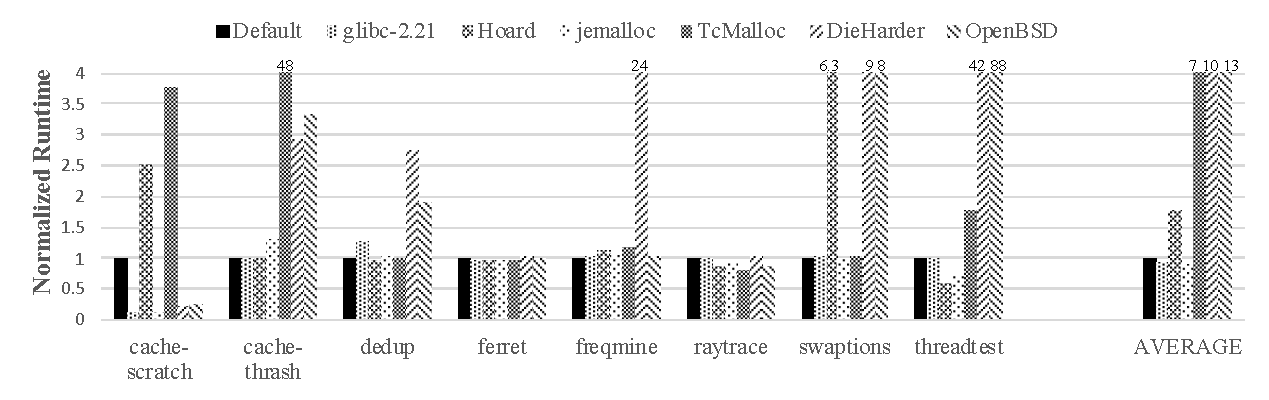
\includegraphics[width=\columnwidth]{figures/regular-performance}
\caption{Performance Difference with Different Allocators\label{fig:motivation}}
\end{figure}

%Are all profilers combined together could figure out the performance issues? No, since they are not differentiated between memory management operations. Also, they cannot identify the issues caused by kernel contention.

Although memory allocators have a significant impact on performance and memory overhead, none of existing profilers can actually report these issues. Existing allocation profilers, such as \texttt{mprof}~\citep{Zorn:1988:MAP:894814}, Mtrace~\citep{mtrace}, Mtrace++~\citep{Lee:2000:DMM:786772.787150}, \texttt{TcMalloc} profiler~\citep{tcmalloc-profiler}, or CLR profiler~\citep{lupasc2014dynamic}, mainly focus on how an application uses the memory, instead of identifying the inherent design issues of the allocators. For instance, \texttt{mprof} attributes memory allocations to different allocation sites, and reports memory leaks and a direct allocation table that shows the memory usage of functions~\citep{Zorn:1988:MAP:894814}. The \texttt{TcMalloc} profiler reports heap usage of different allocation sites, and locates memory leaks~\citep{tcmalloc-profiler}. However, they cannot identify the performance and memory issues inside an allocator itself. 

General profilers, such as gprof~\citep{DBLP:conf/sigplan/GrahamKM82}, Coz~\citep{Coz}, and perf~\citep{perf}, report the time accumulation of different functions, while Coz can further present quantitative performance impact by improving a particular region of code. However, they cannot identify performance issues of a memory allocator, due to the following reasons. \texttt{First}, they do not collect allocator-specific data, and provide no metrics for evaluating an allocator. For instance, \texttt{perf} may report the number of cache misses, but it is impossible to know how many of these events are actually caused by the allocator. Without that information, it is unable to determine whether a performance issue is originating from the allocator. \texttt{Second}, none of these tools collect kernel contention information, an important issue related to the allocator. For instance, the glibc-2.21 allocator slows down the performance of \texttt{dedup} by more than 20\%, which is caused by frequent \texttt{madivse} system calls that directly lead to the heavy kernel contention. However, such an important issue cannot be identified by general profilers~\citep{DBLP:conf/sigplan/GrahamKM82, Coz, perf}%, \todo{as discussed in Section~\ref{}}.
Third, none of these profilers report the application friendliness of an allocator, which is critical to understanding the performance slowdown caused by a particular allocator.   

This paper proposes \MP{}, the \textbf{first} general allocator profiler to profile different memory allocators. \textbf{\MP{} not only helps allocator programmers, but also benefits normal programmers and users}. \textit{First, it provides multiple metrics that help allocator developers to discover design issues of a particular memory allocator}. \textit{Second, it helps normal programmers to determine whether an application's performance or scalability issue is caused by a memory allocator}. 
%\MP{} reports multiple metrics for users to judge whether the allocator is the culprit of the performance/scalability issue or not. 
If so, programmers can fix the issues affecting the allocator or switch to a better-suited allocator altogether, instead of focusing on the application itself. 
\textit{Third, mmprof reports different types of memory overhead caused by an allocator, helping normal users analyze memory overhead issues.} 
%Existing allocator profilers only reports memory usage/leaks from application code~\cite{mprof, Zorn:1988:MAP:894814, mtrace, Lee:2000:DMM:786772.787150, tcmalloc-profiler, lupasc2014dynamic}, which are complementary to \MP{}. 
If the memory overhead is mainly caused by an allocator, e.g., TcMalloc uses $1.8\times$ more memory than the default Linux allocator for \texttt{swaptions}, then it is less useful to reduce the memory usage of this application. Instead, a more memory-efficient allocator should be employed.   


% What to do? and How to do?
\MP{} aims to evaluate all important aspects of memory allocators, such as performance, memory, scalability, and application-friendliness. \MP{} is based on the observation that memory allocators share many commonalities, making it feasible to design a general profiler for different allocators. First, they interact with other components of the system similarly: they provide the same API's to applications (e.g., \texttt{malloc()} and \texttt{free()}), invoke a limited set of system calls (e.g., \texttt{mmap} and \texttt{sbrk}), and employ a set of thread synchronization primitives for synchronization. Second, memory allocators share similar memory management policies, such as belonging to either sequential or BiBOP-style memory layout types, employing per-thread heaps, differentiating small and large objects, and managing small objects with different size classes (where more details are discussed in Section~\ref{sec:allocator}). Therefore, \textit{mmprof employs several common mechanisms to perform the profiling, while utilizing a configuration file to understand the differences between various allocators}.    

\MP{} intercepts the interactions between an allocator and other components such as the application, the \texttt{pthreads} library, and the underlying operating system, in order to collect the detailed data for each allocation/deallocation request, and the contention information for both user and kernel space. 
 \MP{} employs simple counters and timestamps for collecting basic data, such as the number of invocations. In addition, \MP{} further employs the CPUs' Performance Monitoring Units (PMU's) to collect hardware-based events, and attributes them each to allocations/deallocations. The PMU's avoid the requirement of explicitly modify source code, and provide more insights about a particular design issue. \MP{} also proposes practical solutions to evaluate certain important metrics, such as cache/page utilization rates, memory blowup, active/passive false-sharing, and kernel contention. Although some of these metrics have been proposed before~\cite{Hoard}, \textit{mmprof is the first to evaluate them quantitatively}. In order to enable the comparison between different executions, \MP{} normalizes the data to each allocation, each access, and each unit of time.  

% How we are going to implement this? 
%\MP{} uses the hardware Performance Monitor Units (PMU) and RDTSC timestamps widely available in modern CPUs to perform the profiling. \MP{} achieves three goals to act as a practical memory allocator profiler for real-world programs. First, it should directly work on the executables. Second, it should reveal the overhead and scalability of the allocators themselves. Since the invocations to the memory management functions are synchronous, the efficiency of the allocator has a direct impact on performance. Third, it should quantify the ``application friendliness'' of the memory allocator, a metric to show how well the allocator manages memory for the application, which is drawn from statistics of accesses to different levels of the memory hierarchy.

%(1) When the profiler works directly on the executable, it is difficult to distinguish the behaviors caused by the allocators and those caused by the program code. 
%We face multiple challenges to achieve the goals. (1) The profiler, despite sampling a large number of events and obtaining extensive information, should maintain a low runtime overhead, and should not seriously distort the execution of the profiled targets (e.g. allocator).  (2) The profiler should not only identify the regular design issues (e.g., poor cache locality or poor object reuses) of the allocator, but also reveal the serious issue of interacting with the OS since a poor design may invoke excessive OS system calls and introduce unnecessary kernel contention. (3) A memory allocator may significantly affect the performance of applications, not just limiting to itself, which has never been evaluated quantitively before. (4) The profiler should be able to adapt to different allocators, which is the major target of designing a general profiler.   
%  to be quantified. 
% manage memory outside of its library calls, which is hard to capture and quantify. 
%carefully manage its internal memory allocations to

%To address these challenges, we design \MP{} in a principled way to determine what events to sample and what profile knowledge the sampled events contribute to. Briefly speaking, \MP{} always intercepts the allocator library calls to figure out when the program execution is inside the allocator, during which it samples both performance related PMU events (e.g., cache misses) to determine the implementation issues and intercepts OS kernel calls to understand OS-level contention. When the program execution is outside of the allocator, \MP{} samples specific PMU events to determine cache line- and page-level utilization ratio, and cache contention rate, which could directly and significantly impact the performance of the corresponding applications. To maintain low overhead, \MP{} employs a fast lookup mechanism that enables fast checking on the size information of each object, and on the cache line usage and page usage upon each sampled access. ??(WB) one more sentence about the low overhead?? ??(WB) It allocates its internal memory on ...??

Based on our extensive evaluation, \MP{} successfully identifies multiple design/implementation issues found inside popular allocators, as further described in Section~\ref{sec:effectiveness}. \MP{} also provides metrics to evaluate the performance, memory overhead, scalability, and application-friendliness of an allocator, which can serve as a basis when developing a new allocator. Due to its careful design, \MP{}'s performance overhead is around $2.5\times$, its memory overhead is around $56\%$, all while sampling a large number of events and collecting a large amount of information. This efficient design reduces \MP{}'s interference to the original execution. 

%\todo{one way to highlight the contribution is to emphasize on the **complex** considerations of designing good allocators and the challenges to identify design problems. We want to let the reviewer know that it's difficult to do. }

\subsection*{Contribution}

Overall, this paper makes the following contributions. 

\begin{itemize}
\item It proposes the first general profiler--\MP{}--to profile different memory allocators, without the need for changing allocators and applications.  

\item \MP{} employs CPU Performance Monitoring Units (PMU's), time-stamp counters, and simple counters acting together to profile allocators quantitatively. 

\item \MP{} collects a range of metrics to evaluate memory allocators, and proposes practical methods to profile some of them quantitatively for the first time. 
%profile cache/page utilization rate, memory blowup, active/passive false sharing, and kernel contention for the first time.
%, and attributes the data to each allocation and deallocation, helps discover designing issues that cannot be discovered with general profilers.  
 
\item This paper performs extensive experimentation to confirm its effectiveness, performance, and memory overhead.    

\end{itemize} 

\begin{comment}

%\todo{What is new in this tool? Whether it could provide some information that is not available in an existing allocator.}

\begin{itemize}
\item It will quantify application-friendliness, which is not available in existing work, and which helps users to decide which allocator should be used for a specific application. 
\item It will provide the memory usage (overhead) information, such as internal fragmentation, and objects that are not freed but yet which remain unused. 
\item It will provide some information that only exists across multiple profilers, for instance, the average number of instructions of each allocation and deallocation, the average time spent within each allocation and deallocation (PMU sampling will be placed outside of the time span, thus not avoiding an erroneous measurement of how long this allocation and deallocation request has been sampled), whether there are some contentions during allocation (user space and kernel space), how many lock acquisitions.  
\end{itemize}
 	
\end{comment}

\subsection*{Outline}

The remained of this paper is organized as follows. Section~\ref{sec:background} discusses the background of memory allocators, and the basic idea and challenges of \MP{}. Then Section~\ref{sec:implementation} presents the detailed implementation. After that, Section~\ref{sec:evaluation} shows the results of experiments on different allocators using \MP{}, and Section~\ref{sec:limitation} discusses some limitations. In the end, Section~\ref{sec:relatedwork} discusses related work in this field, and Section~\ref{sec:conclusion} concludes this paper.